\documentclass[conference]{IEEEtran}
\IEEEoverridecommandlockouts
% The preceding line is only needed to identify funding in the first footnote. If that is unneeded, please comment it out.
\usepackage{cite}
\usepackage{amsmath,amssymb,amsfonts}
\usepackage{algorithmic}
\usepackage{graphicx}
\usepackage{textcomp}
\usepackage{xcolor}
\def\BibTeX{{\rm B\kern-.05em{\sc i\kern-.025em b}\kern-.08em
    T\kern-.1667em\lower.7ex\hbox{E}\kern-.125emX}}
\begin{document}

\title{ME547MidtermReport}
\author{Tyler Allen Freitas}
\date{January 2024}

\title{ME547 Midterm Report: \\ Modeling and Simulating a Vectored Thrust Aircraft}

\author{\IEEEauthorblockN{Tyler Freitas}
\IEEEauthorblockA{\textit{ME547 student} \\
\textit{University of Washington}\\
Seattle, WA, USA \\
tfreita@uw.edu}
}

\maketitle

\begin{abstract}
The following analysis models a 2D vectored thrust aircraft and simulates its positional response with different thruster inputs. This nonlinear model is derived from Newtons' laws of motion and linearized around its equilibrium points using Jacobian Linearization and small angle approximation. The simulation tested a step, impulse, and sinusoidal inputs to determine the aircraft positional response. The simulation showed the aircraft horizontal position is unstable for all inputs because the aircraft orientation increases beyond its small angle approximation, and the aircraft model neglects air torque resistance. The vertical position was stable for an impulse input but not asymptotic stable for a step and sinusoidal inputs. The next course of action for this analysis will be implementing a Linear-Quadratic Regulator (LQR) controller to maintain stability.
\end{abstract}


\section{Introduction}
The study of motion controls can be explored in many mechanical system applications. Motion controls have been implemented on aircraft for many years to control structural components including ailerons, elevators, and rudders. In recent decades, the Harrier jump jet has introduced the possibility for vertical takeoff and landing [1]. Specifically, this aircraft can hover and vertically takeoff \& land by changing the direction of the thrusters from a horizontal to downward position [1]. To navigate these vertical maneuvers, a controller is implemented for positional stability [3],[1]. This paper will focus on creating a model and simulating the response of a hovering vectored thrust aircraft.  

\section{Problem Formation:}
\subsection{Model/Plant}
The model (plant) of this system is a vectored thrust aircraft, which is analyzed as a rigid body in a 2D space. This model has 3 thrusters: 1 thruster passing through the aircraft centroid, and 2 angled thrusters  near the wingtips [1]. Note that these wingtip thrusters are used for aircraft stability [1]. These 3 thrusters are coupled together and move as an unit. Therefore, the changes of the wingtip thruster angles are the same. Fig. 1 displays the free body diagram  (FBD) of the plant.  This diagram is in the Cartesian coordinates system. The outputs of the system are the position ($X$, $Y$) and orientation ($\theta$) of the aircraft. Note that the simulation outputs are only the horizontal ($X$) and vertical ($Y$) positions. The reaction forces of the thrusters are translated to a common intersection point, and $r$ is the distance from this common intersection point of the thrusters to the aircraft centroid [1]. Additionally, these reaction forces are combined and broken-down to its horizontal ($F_1$) \& vertical ($F_2$) components which are the inputs for this plant. The other arrows in this FBD are the applied thruster forces. Note that this FBD neglects the air drag forces.

\subsection{Free-Body Diagram}
\begin{figure}[!htbp]
\centerline{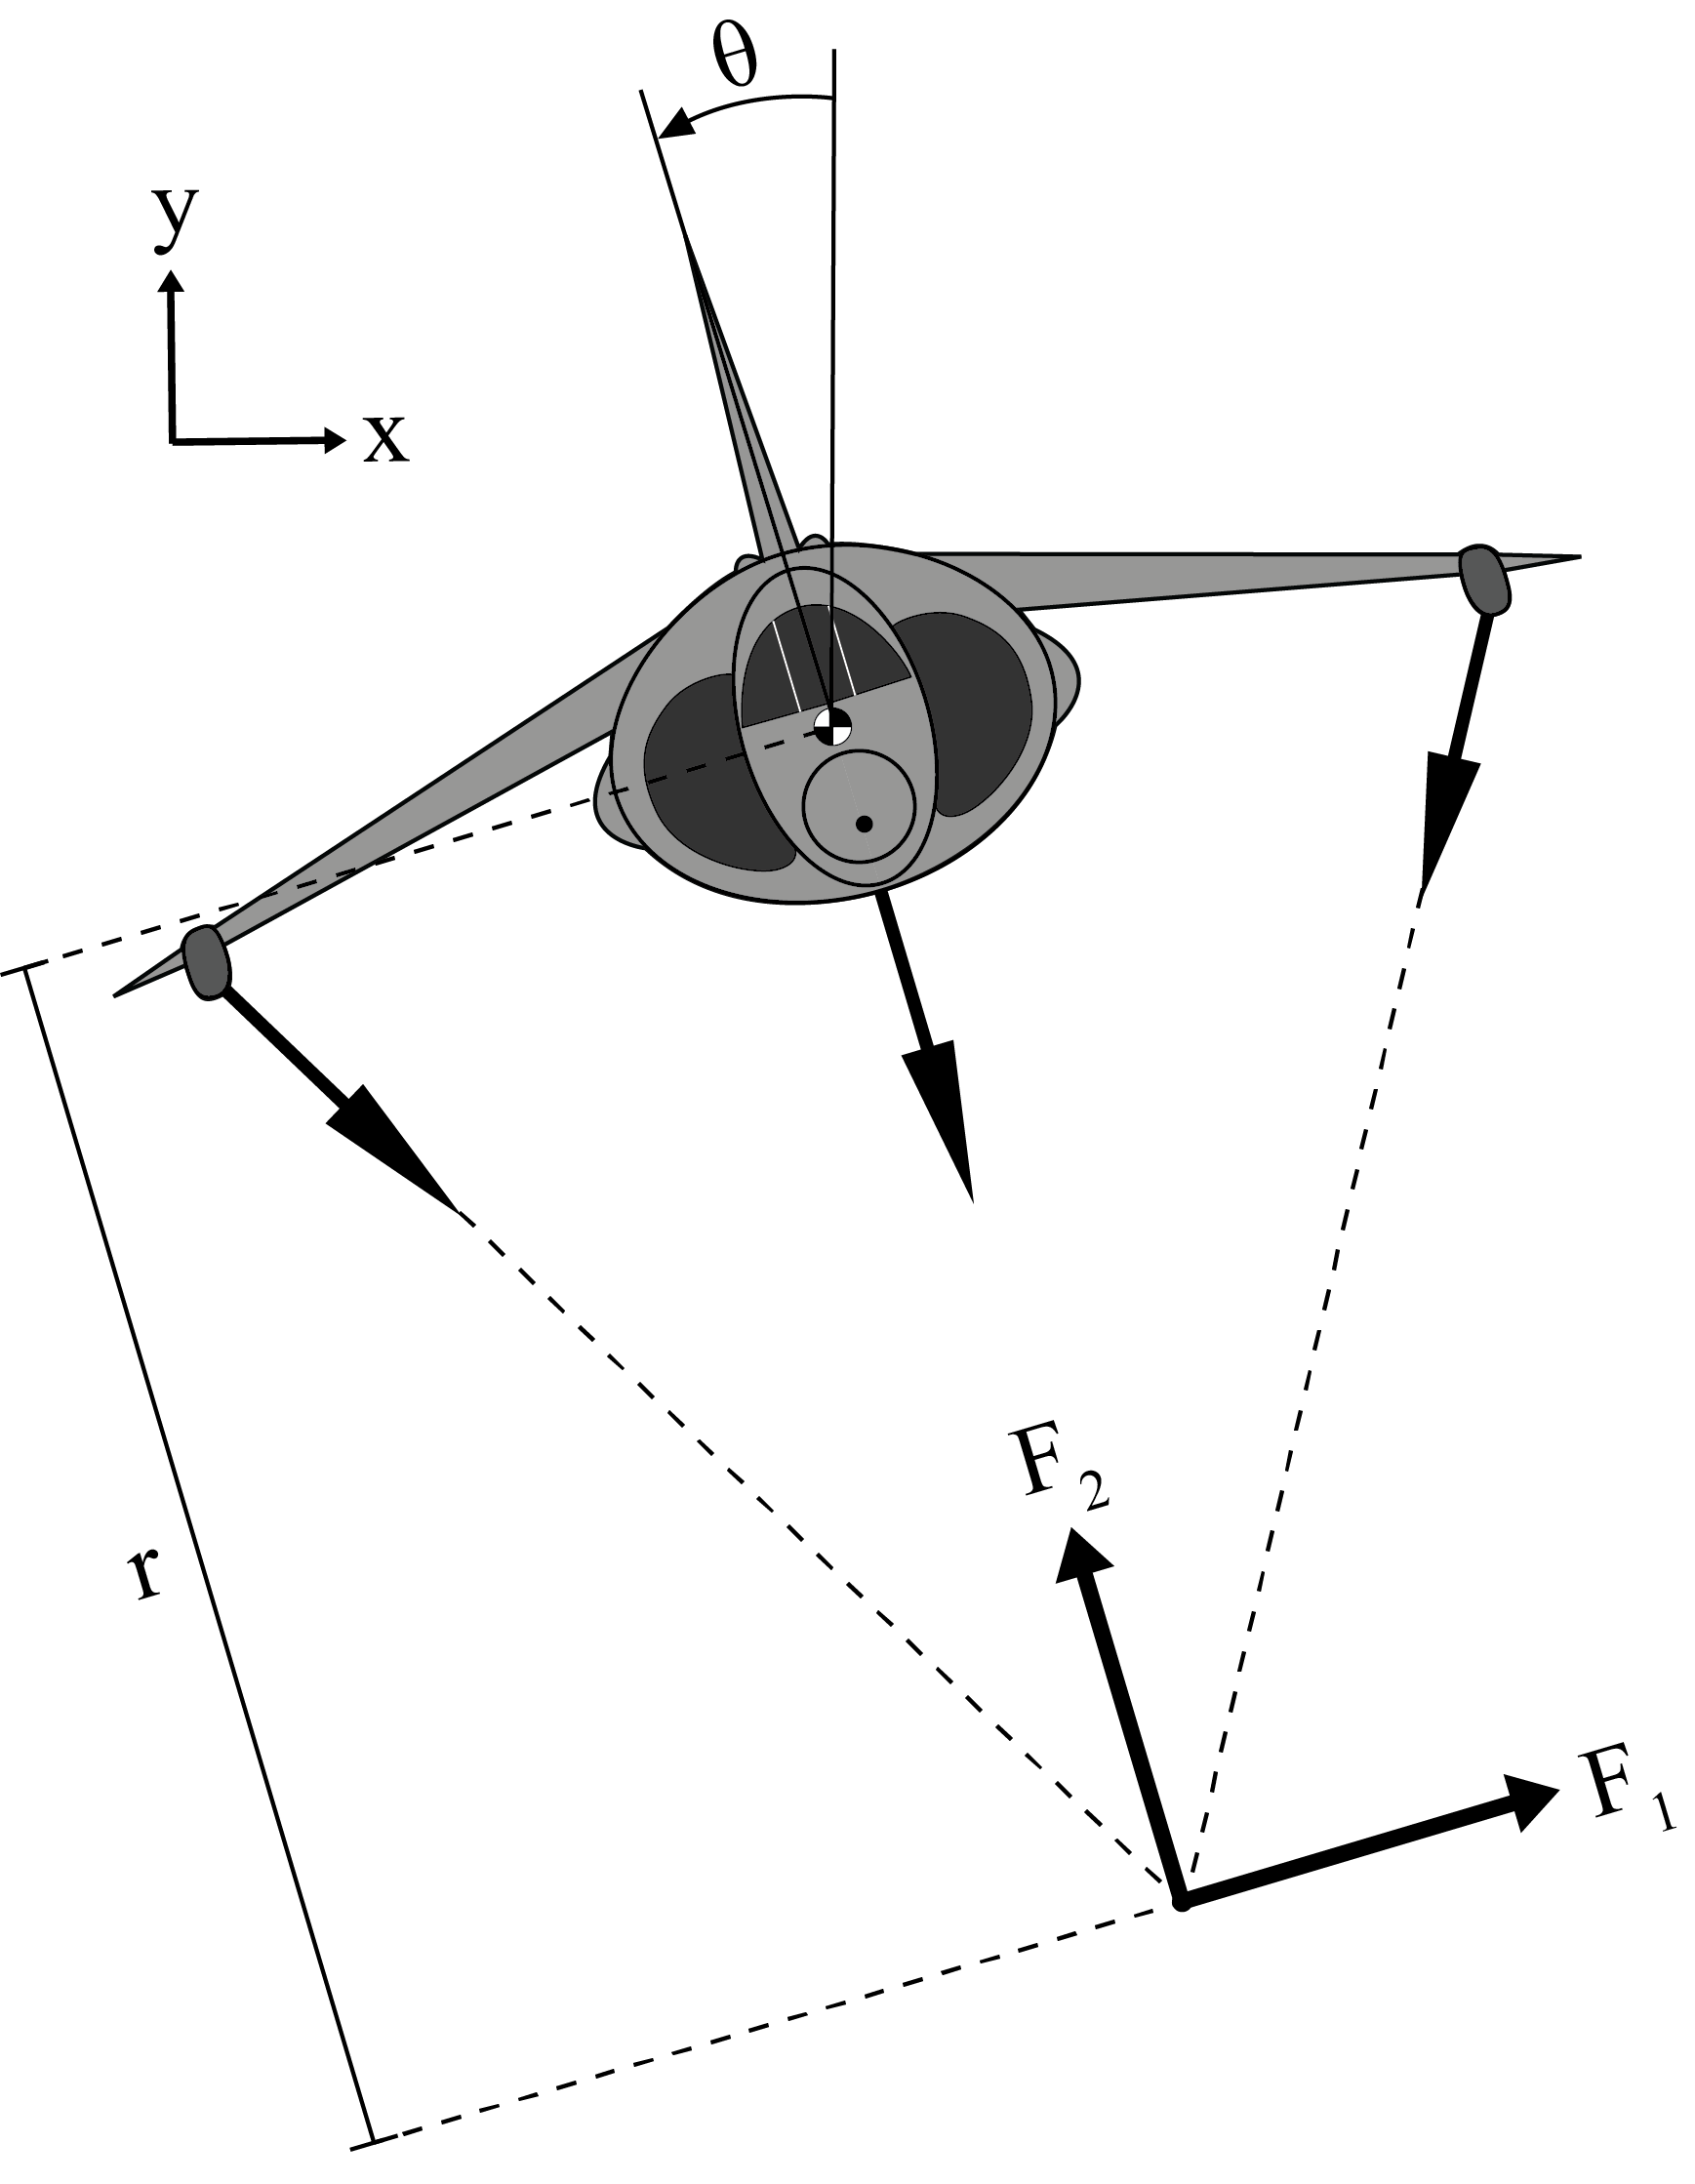
\includegraphics[scale = 0.40]{547_Midterm_FBD_bkg.png}}
\caption{2D Vectored Thrust Aircraft Free Body Diagram}
Note: This diagram is not to scale.
\label{figure1}
\end{figure}

\subsection{Phyiscs:}
The aircraft can be represented as an airfoil which experiences aerodynamic forces (lift \& drag) from the air pressure distribution and shear stresses. The lift force counteracts the weight of the aircraft, and the thrust reduces the drag. Based on Newton’s $3^{rd}$ law, the applied downward thruster forces will have equal and opposite reactions, which are the aircraft lift forces. Also, the differential pressures across the aircraft area will create lift. The weight of the system is the aircraft mass. Drag is created by air and the vertical thruster reaction ($F_2$) in the drag direction. The air stream is a laminar flow because the vertical maneuvers of the aircraft are at low speeds. The translational air drag, which opposites the direction of motion, is equal to the velocity times the damping coefficient ($F_{drag} = cx^\prime$). Note that the $1^{st}$ derivative of the aircraft position is velocity. The air drag coefficient ($c$) is depend on the frictional forces from the shear stresses along the surface of the aircraft and the air pressure distribution in the drag direction.\\

Newton's $2^{nd}$ law of motion is valid for this dynamic model because the position and orientation of the aircraft change in time, not in space. This law states the summation of forces equal the mass times acceleration. Similarly, the summation of torques equal the moment of inertia times angular acceleration. Note that the $2^{nd}$ derivative of position is the aircraft acceleration. Based on the FBD in Fig. 1, the system forces are air drag, reaction forces by the thrusters, and weight. These forces are broken down into their respected x and y components (Equations 1 \& 2). Note that these model equations are applicable to a hovering aircraft with no external disturbances. For Equation 3, the only torque on the aircraft is from the thruster reaction ($F_1$). Note that there is no air torque resistance in Equation 3.

\subsection{Nonlinear Differential Equations [1]:} 
\[
mx^{\prime\prime} = F_1cos\theta - F_2sin\theta - cx^{\prime}  \tag{1}
\] 
\[
my^{\prime\prime} = F_1sin \theta + F_2cos\theta - mg - cy^\prime \tag{2}
\]
\[
J\theta^{\prime\prime} = rF_1 \tag{3} 
\]\\
Fig. 2 shows a nonlinear block diagram in Simulink. \\
Note: $u_1$ and $u_2$ represent $F_1$ and $F_2$ respectively in this block diagram. \\

\begin{figure}[!h]
\centerline{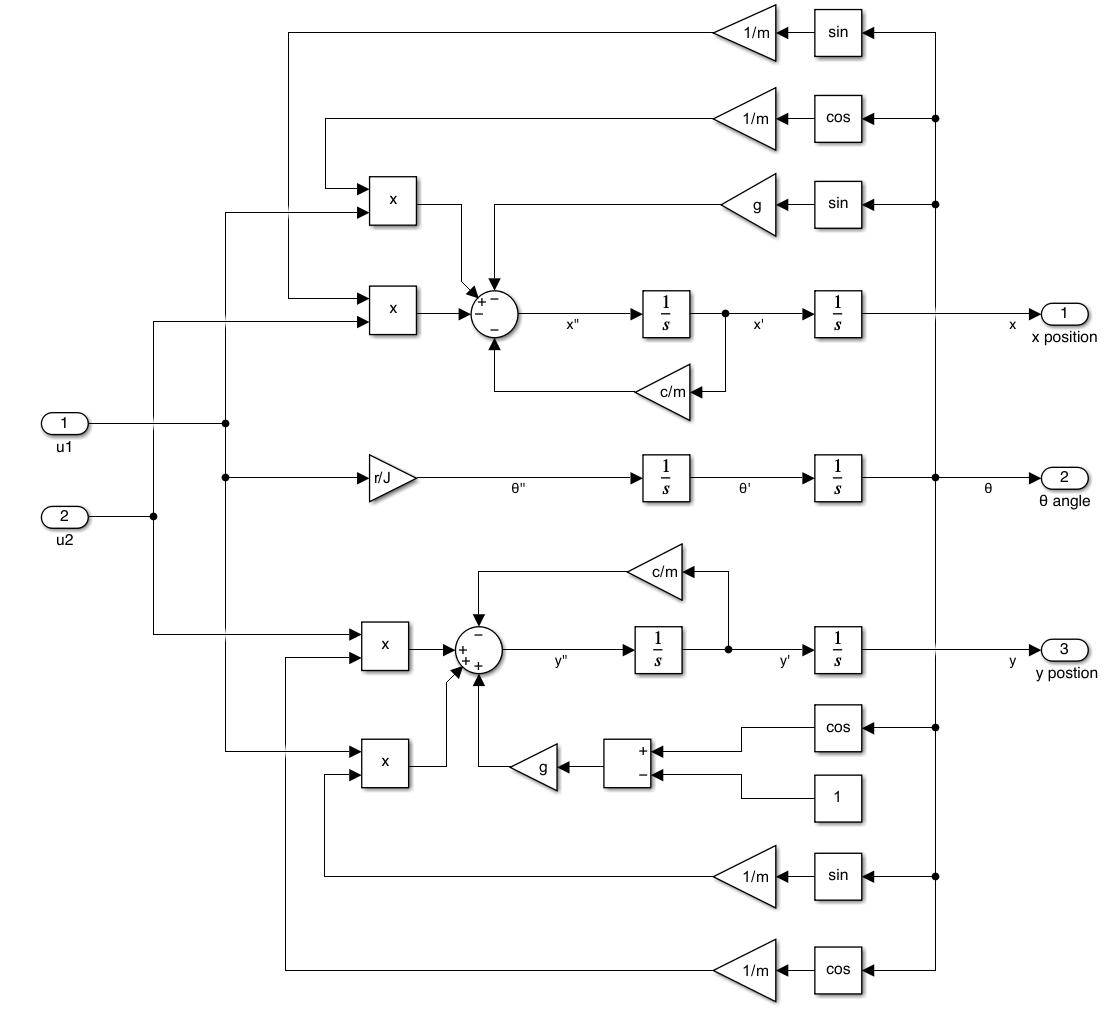
\includegraphics[scale=0.35]{non-linear_Block_Diagram.png}}
\caption{Nonlinear Block Diagram}
\label{figure}
\end{figure}

\subsection{Nonlinear Differential Equation Observations:}
This model has three coupled $2^{nd}$ order, ordinary differential equations. Note that these nonlinear equations have trigonometric functions. This system of equations is a continuous time model and a time varying system because the response and the differential equation coefficients depend on time. The model is casual because the equations depend on the current states. This is a dynamic system as the aircraft position and orientation change respect to time.\\ 

Table 1 lists the mathematical variables used in this analysis.
\begin{table}[htbp]
\begin{center}
\caption{Mathematical Variables}
\begin{tabular}{|c|c|c|}
\hline
\textbf{\textit{Variables}}& \textbf{\textit{Variable Name}}& \textbf{\textit{Units}} \\
\hline
$x$ & aircraft horizontal position & $m$ \\
\hline
$x'$ & aircraft horizontal velocity & $m/s$ \\
\hline
$x''$ & aircraft horizontal acceleration & $m/s^2$ \\
\hline
$y$ & aircraft vertical position & $m$ \\
\hline
$y'$ & aircraft vertical velocity & $m/s$ \\
\hline
$y''$ & aircraft vertical acceleration & $m/s^2$ \\
\hline
$\theta$ & aircraft angular position & $rad$ \\
\hline
$\theta'$ & aircraft angular velocity & $rad/s$ \\
\hline
$\theta''$ & aircraft  angular acceleration & $rad/s^2$ \\
\hline
$J$ & moment of inertia & $kg*m^2$ \\
\hline
$r$ & distance from aircraft centroid to thrusters intersection& $m$ \\
\hline
$c$ & damping coefficient & $Ns/m$ \\
\hline
$g$ & acceleration due to gravity  & $m/s^2$ \\
\hline
$m$ & aircraft mass & $kg$ \\
\hline
$F_1$ & aircraft horizontal reaction & $N$ \\
\hline
$F_2$ & aircraft vertical reaction & $N$ \\
\hline
$y_e$ & y equilibrium point & $m$ \\
\hline
$x_e$ & x equilibrium point & $m$ \\
\hline
$z_e$ & state-space equilibrium points & $-$ \\
\hline
$F_e$ & input equilibrium points & $N$ \\
\hline
$A,B,C,D$ & state-space matrices & $-$ \\
\hline
$\zeta$ & linearized state-space variable & $-$\\
\hline
$v$ & linearized state-space input & $-$\\
\hline
$P$ & linearized state-space output & $-$\\
\hline
$z$ & nonlinear state-space variable & $-$\\
\hline
$f$ & time derivative of z & $-$\\
\hline
$h$ & nonlinear state-space output & $-$\\
\hline
$F$ & nonlinear state-space input & $-$.\\
\hline
$G_1$ & Local x transfer function & $-$\\
\hline
$G_2$ & Local y transfer function & $-$\\
\hline
\end{tabular}
\end{center}
\end{table}

\newpage
\section{Analysis}
This model is a system of nonlinear differential equations. Therefore, the system will be linearized around its equilibrium points with the Jacobian Linearization method [2]. These $2^{nd}$ differential equations are converted to a nonlinear state-space system, which is a system of $1^{st}$  order differential equations. z is the nonlinear state-space variable for the state equations: ($z$ = ($z_1 = x$, $z_2 = y$, $z_3 = \theta$, $z_4 = x^\prime$, $z_5 = y^\prime$, \& $z_6 = \theta^\prime$)), and F is the nonlinear input variable: ($F$ = ($F_1,F_2$)).\\

Note: assume small angle approximation around the equilibrium points: $sin(\theta) \approx \theta$ \& $cos(\theta) \approx 1$. The range of $\theta$ is from 0 to $2\pi$. Equations 4 and 5 show the nonlinear state-space and output equations respectively [1]. $f$ is the time derivative of $z$, and $h$ is the nonlinear state-space output.

\[
f(z,F) = \frac{dz}{dt} =
\begin{pmatrix}
z_4\\
z_5\\
z_6 \\
-\frac{c}{m}z_4 + \frac{F_1}{m} -\frac{F_2z_3}{m}\\
-g - \frac{c}{m}z_5 + \frac{F_1z_3}{m} +\frac{F_2}{m}\\
\frac{r}{J}F_1\\
\end{pmatrix}  
\tag{4}
\]

\[
h = 
\begin{pmatrix}
z_1\\
z_2\\
\end{pmatrix}
\tag{5}
\]\\

\subsection{Finding the Equilibrium Points:}
The equilibrium points are determined by setting these nonlinear system of equations (Equations 4 \& 5) to zero and solving for each $z$ and $F$ variable. \\

\noindent Stable Equilibrium Points: \\
\indent $z_e$ = ($z_1 = x_e$, $z_2 = y_e$, $z_3 = 0$, $z_4 = 0$, $z_5 = 0$, $z_6 = 0$)\\
\indent $F_e$ = ($F_1 = 0$, $F_2 = mg$)\\
Note: the system of equations above are independent of $x$ and $y$. \\

At a given equilibrium point ($x_e$ \& $y_e$), there is no rotational or translational velocity, and the horizontal reaction force ($F_1$) and $\theta$ are zero. The vertical reaction force ($F_2$) supports its own weight. 

\subsection{Jacobian Matrices:}
Equations 6 and 7 compute the Jacobian Matrices for this nonlinear system [1].
\[ 
A = \frac{\partial f}{\partial z}\bigg|_{(z_e,F_e)}
B = \frac{\partial f}{\partial F}\bigg|_{(z_e,F_e)}
\tag{6}
\]
\[ 
C = \frac{\partial h}{\partial z}\bigg|_{(z_e,F_e)}
D = \frac{\partial h}{\partial F}\bigg|_{(z_e,F_e)}
\tag{7}
\]

\newpage
The following 8-11 equations breakdown the Jacobian Matrices into the partial derivatives of $f$ and $h$ in respect to the nonlinear state-space variable ($z$) and nonlinear state-space input ($F$).

\[
A = 
\begin{bmatrix}
\frac{\partial f_1}{\partial z_1}&\frac{\partial f_1}{\partial z_2}& \frac{\partial f_1}{\partial z_3}& \frac{\partial f_1}{\partial z_4}& \frac{\partial f_1}{\partial z_5} &\frac{\partial f_1}{\partial z_6}\\\\
\frac{\partial f_2}{\partial z_1}&\frac{\partial f_2}{\partial z_2}& \frac{\partial f_2}{\partial z_3}& \frac{\partial f_2}{\partial z_4}& \frac{\partial f_2}{\partial z_5} &\frac{\partial f_2}{\partial z_6}\\\\
\frac{\partial f_3}{\partial z_1}&\frac{\partial f_3}{\partial z_2}& \frac{\partial f_3}{\partial z_3}& \frac{\partial f_3}{\partial z_4}& \frac{\partial f_3}{\partial z_5} &\frac{\partial f_3}{\partial z_6}\\\\
\frac{\partial f_4}{\partial z_1}&\frac{\partial f_4}{\partial z_2}& \frac{\partial f_4}{\partial z_3}& \frac{\partial f_4}{\partial z_4}& \frac{\partial f_4}{\partial z_5} &\frac{\partial f_4}{\partial z_6}\\\\
\frac{\partial f_5}{\partial z_1}&\frac{\partial f_5}{\partial z_2}& \frac{\partial f_5}{\partial z_3}& \frac{\partial f_5}{\partial z_4}& \frac{\partial f_5}{\partial z_5} &\frac{\partial f_5}{\partial z_6}\\\\
\frac{\partial f_6}{\partial z_1}&\frac{\partial f_6}{\partial z_2}& \frac{\partial f_6}{\partial z_3}& \frac{\partial f_6}{\partial z_4}& \frac{\partial f_6}{\partial z_5} &\frac{\partial f_6}{\partial z_6}
\end{bmatrix}
\Bigg|_{(z_e,F_e)} 
\tag{8}
\] 

\[
B = 
\begin{bmatrix}
\frac{\partial f_1}{\partial F_1}&\frac{\partial f_1}{\partial F_2} \\\\
\frac{\partial f_2}{\partial F_1}&\frac{\partial f_2}{\partial F_2} \\\\
\frac{\partial f_3}{\partial F_1}&\frac{\partial f_3}{\partial F_2} \\\\
\frac{\partial f_4}{\partial F_1}&\frac{\partial f_4}{\partial F_2} \\\\
\frac{\partial f_5}{\partial F_1}&\frac{\partial f_5}{\partial F_2}\\\\
\frac{\partial f_6}{\partial F_1}&\frac{\partial f_6}{\partial F_2}
\end{bmatrix}
\Bigg|_{(z_e,F_e)} 
\tag{9}
\] 

\[
C = 
\begin{bmatrix}
\frac{\partial h_1}{\partial z_1}&\frac{\partial h_1}{\partial z_2}& \frac{\partial h_1}{\partial z_3}& \frac{\partial h_1}{\partial z_4}& \frac{\partial h_1}{\partial z_5} &\frac{\partial h_1}{\partial z_6}\\\\
\frac{\partial h_2}{\partial z_1}&\frac{\partial h_2}{\partial z_2}& \frac{\partial h_2}{\partial z_3}& \frac{\partial h_2}{\partial z_4}& \frac{\partial h_2}{\partial z_5} &\frac{\partial h_2}{\partial z_6}
\end{bmatrix}
\Bigg|_{(z_e,F_e)} 
\tag{10}
\] 
\[
D =
\begin{bmatrix}
\frac{\partial h_1}{\partial F_1}&\frac{\partial h_1}{\partial F_2} \\\\
\frac{\partial h_2}{\partial F_1}&\frac{\partial h_2}{\partial F_2}
\end{bmatrix}
\Bigg|_{(z_e,F_e)} 
\tag{11}
\] 

\newpage
\subsection{Linearized State-Space Equations \& Block Diagram:}
These Jacobian Matrices (Equations 14-17) create a linearized state-space system, which analyze the local behavior around the equilibrium points [1]. New variables are created by subtracting the nonlinear state-space variable and input with its equilibrium points. Thus, $\zeta = z - z_e$\, which is the linearized state-space variable, $v = F - F_e$, which is the linearized state-space input variable, and P is the linearized state-space output variable. Equations 12 and 13 show the linearized state-space and output equations respectively [1].

\[
\zeta^\prime = A\zeta + Bv
\tag{12}
\] 
\[
P = C\zeta + Dv
\tag{13}
\] 

\[
A = 
\begin{bmatrix}
0&0& 0& 1& 0 &0\\
0 &0 &0 &0 &1 &0\\
0 &0 &0 &0 &0 &1\\
0 &0 &-g& -c/m &0 &0\\
0 &0 &0 &0 &-c/m &0\\
0 &0 &0 &0 &0 &0\\
\end{bmatrix}
\tag{14}
\]
\[
B = 
\begin{bmatrix}
0 &0\\
0 &0\\
0 &0\\
1/m& 0\\
0 &1/m\\
r/J& 0\\
\end{bmatrix}
\tag{15}
\] 

\[
C = 
\begin{bmatrix}
1&0&0&0&0&0\\
0&1&0&0&0&0\\
\end{bmatrix}
\tag{16}
\]
\[
D =
\begin{bmatrix}
0&0\\
0&0\\
\end{bmatrix}
\tag{17}
\] 

For reference, the following 18-25 equations show each linearized state and output equation.\\ 

Linearized State Equations:
\[
\zeta_1^\prime = x^\prime\tag{18}
\] 
\[
\zeta_2^\prime = y^\prime\tag{19}
\]
\[
 \zeta_3^\prime = \theta^\prime \tag{20}
\]
\[
\zeta_4^\prime = -g\theta -c/mx^\prime + v_1/m \tag{21}
\]
\[
\zeta_5^\prime = -c/my^\prime + v_2/m \tag{22}
\]
\[
\zeta_6^\prime = (r/J)v_1 \tag{23}
\]

Linearized Output Equations:
\[
P_1 = \zeta_1 = x - x_e \tag{24}
\]
\[
P_2 = \zeta_2 = y - y_e \tag{25}
\]

\newpage
Fig. 3 displays a linearized block diagram in Simulink. \\
Note: $u_1$ and $u_2$ represents $F_1$ and $F_2$ respectively in this block diagram. \\

\begin{figure}[htbp!]
\centerline{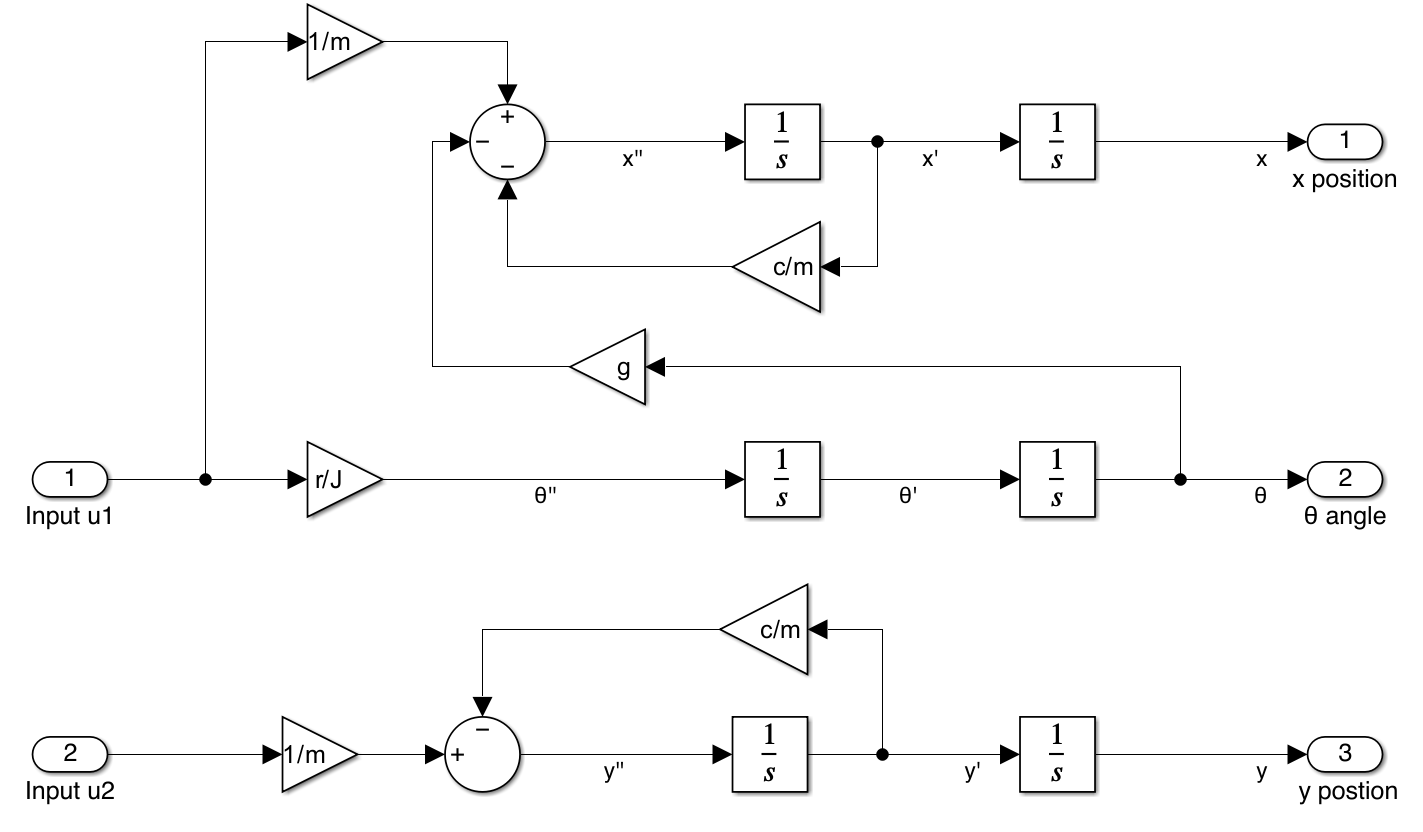
\includegraphics[scale=0.3]{LinearBlock.png}}
\caption{Linearized Block Diagram}
\label{figure}
\end{figure}

\section{Simulation}
The simulation outputs are the local behaviors of the horizontal ($x - x_e$) and vertical ($y - y_e$) aircraft position responses around its equilibrium points. As previously mentioned, this simulation will start at its equilibrium point ($x_e$, $y_e$), and the aircraft is already supporting its own weight at this location. The origin of this equilibrium point is ($x_e = 0$, $y_e = 0$). Note that a sine wave at high \& low frequencies, impulse, and step are the test inputs for this simulation. \\

The following parameters are used in this simulation:
\begin{table}[h]
\begin{center}
\caption{Simulation Parameters [1]}
\label{thelabel}
\begin{tabular}{ |c|c| } 
\hline
m	& 4	$kg$\\
\hline
c	&0.05 $Ns/m$\\
\hline
g	 &9.81 $m/s^2$\\
\hline
J	&0.0475	$kgm^2$\\
\hline
r&	0.25 $m$\\
\hline
$\omega_{low}$&	0.01 $rad/s$\\
\hline
$\omega_{high}$&	1000 $rad/s$\\
\hline
\end{tabular}
\end{center}

\end{table}

\newpage
\subsection{Linearized Transfer Functions, Poles, \& Zeros:}
For this simulation, a MATLAB script converts these linearized Jacobian Matrices to a state-space system and transfer functions. The poles and zeroes are computed to determine the stability and system performance. For each transfer function, a bode plot and the responses of the different inputs are plotted. \\

Matlab converts these state-space equations to a transfer function for each output in the following equation:
\[
 \frac{Y(s)}{U(s)} = C(sI-A)^{-1}B+D \tag{26}
\]

The following shows the poles, zeros, and transfer functions (Equations 27 \& 28) for the local behaviors of the vertical ($y - y_e$) and horizontal ($x - x_e$) positions.\\

Horizontal Position ($x - x_e$) Transfer Function:\\
\[
G_1(s) = \frac{0.25 s^4 + 0.003125 s^3 - 51.63 s^2 - 0.6454 s}{s^6 + 0.025 s^5 + 0.0001563 s^4} \tag{27}
\]
\\
\noindent X Poles: 0, 0, 0, -0.0125, and -0.0125\\
X Zeros: 0, 14.3710, -14.3710, and -0.0125\\

Vertical Position ($y - y_e$) Transfer Function:
\[
G_2(s) = \frac{0.25 s^4 + 0.003125 s^3}{s^6 + 0.025 s^5 + 0.0001563 s^4} \tag{28}
\]
\\
Y Poles: 0, 0, 0, 0, -0.0125, and -0.0125\\
Y Zeros: 0, 0, 0 , -0.0125\\

For both transfer functions, multiple poles at the origin makes this system not asymptotic stable without accounting for pole-zero cancellation. For a step \& impulse input, the local x transfer function has one pole-zero cancellation at the origin, but the multiplicity of the eigenvalues at the origin will cause this system to be unstable. The local y transfer function has 3 pole-zero cancellations at the origin, therefore the system responses will behavior like a $2^{nd}$ order system. For this local y response, the impulse input will be a stable step response, and the step response will behavior like an unstable ramp response. 

\newpage
\section{Results}
The following results are the bode plots and the local behavior of the vertical ($y - y_e$) and horizontal ($x - x_e$) position responses for impulse, step, and a sine wave at different frequencies. 

Note: A sinusoidal output will have the same frequency as the input but shifted in magnitude and phase. For a Bode plot, if the magnitude is greater than 0, the output will be amplified, and when the magnitude is less than 0, the signal will attenuate. The output amplitude is the same as the input amplitude if the magnitude is zero. A negative phase means the output leading the input, and the output lagging the input for a positive phase. The output and input are in-phase when the phase is zero.

\subsection{Local X Responses:}
\subsubsection{Local X Impulse Response} 
\begin{figure}[htbp]
\centering
\centerline{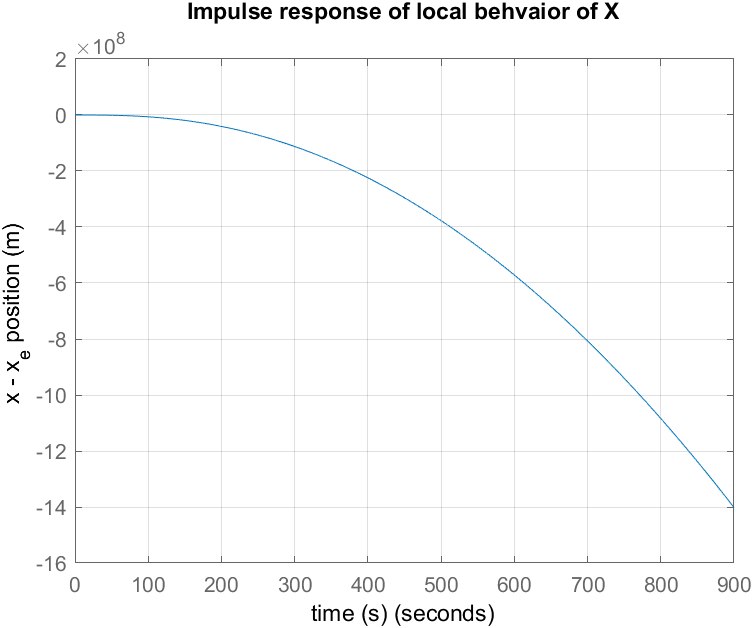
\includegraphics[scale=0.6]{XImpulseRes.png}}
\caption{Impulse X Position Response}
\label{figure}
\end{figure}


Fig. 4 shows the system initially starting at the origin and then going to negative infinity. Based on Equation 21, the impulse input is expected to initially turn the aircraft to the positive x direction, but the magnitude of the air drag and weight component change the trajectory of the system to be in the negative x direction. In the torque equation (Equation 23), the angular acceleration is directly proportional to the input. This equation does not have any torque resistance, so this system will be unstable as $\theta$ increase. The small angle approximation assumption is no longer valid for large angle changes.  

\newpage
\subsubsection{Local X Step Response} 
\begin{figure}[htbp]
\centerline{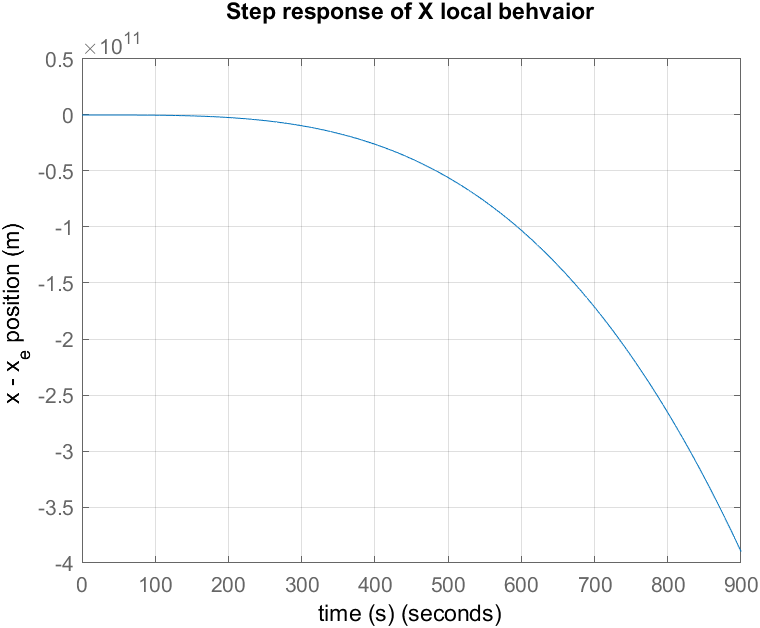
\includegraphics[scale=0.6]{XStepRes.png}}
\caption{Step X Position Response}
\label{figure}
\end{figure}

Fig. 5 describes a similar trend as the impulse response. The step input has a longer constant response than the impulse response initially, but the air drag and gravity component change the trajectory to be unstable as $\theta$ increases. Note that the step input is constant, therefore a constant acceleration will create a parabolic response for local x. The moment of inertia, $J$, is indirectly proportional to the angular acceleration (Equation 23), so a small $J$ will rapidly increase the angular acceleration. Note that this simulation captures the system response for the model and a real aircraft.  

\subsubsection{Local X Bode Response} 
\begin{figure}[htbp]
\centerline{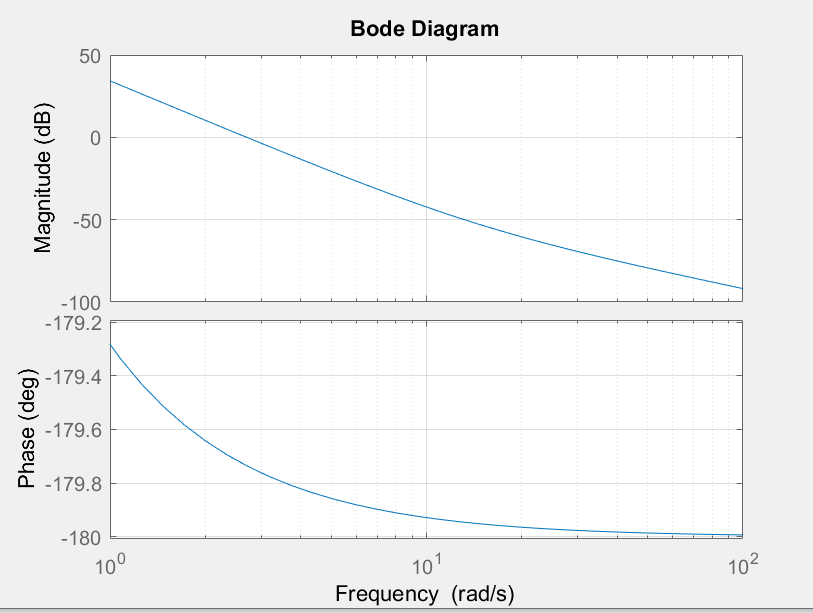
\includegraphics[scale=0.6]{XBode.png}}
\caption{X Bode Plot}
\label{figure}
\end{figure}

In Fig. 6, the magnitude is a constant slope and the phase is an exponential slope for low frequencies. The output magnitude will be amplified, and its phase will be leading the input signal. For high frequencies, the output signal will be leading at a constant -180$^{\circ}$ phase from the input signal, and its magnitude will be attenuating at a smaller slope than the low frequencies. 


\newpage
\subsubsection{Local X High Freq Response}
\begin{figure}[htbp]
\centering
\centerline{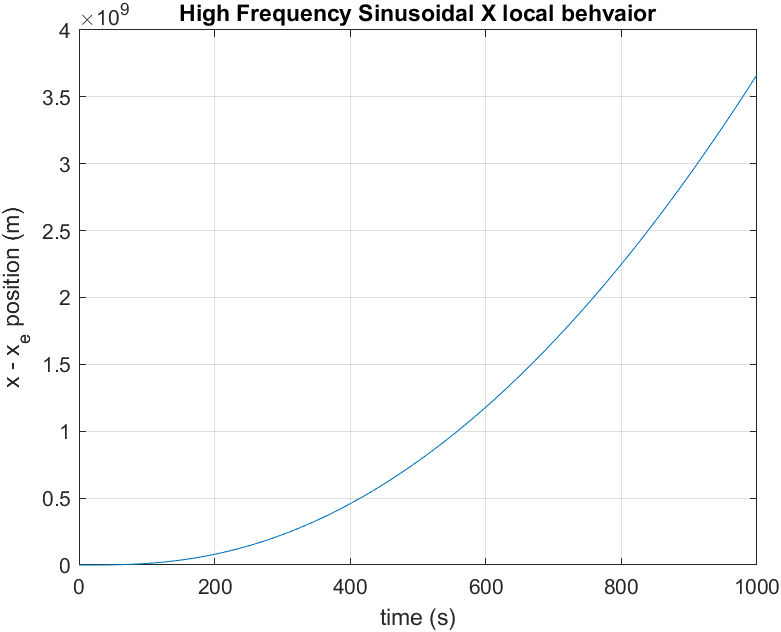
\includegraphics[scale=0.60]{XHighFreqRes.png}}
\caption{High Frequency Sinusoidal X  Position Response}
\label{figure}
\end{figure}

For a high frequency (Fig. 7), the local behavior of x has a similar behavior as the step response. This response agrees with the Bode Plot because the signal attenuates at a smaller slope than the low frequencies response. As previously mentioned, this linearized system will tend to negative infinity as it is unstable. \\

\subsubsection{Local X Low Freq Response} 
\begin{figure}[htbp]
\centerline{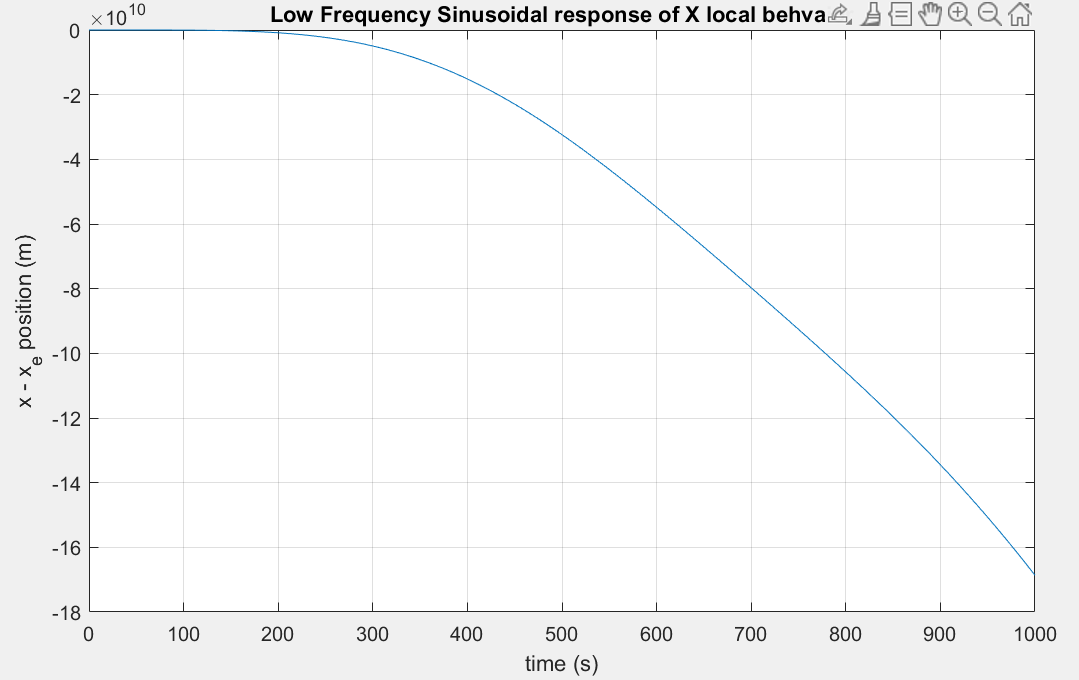
\includegraphics[scale=0.4]{XLowFreqRes.png}}
\caption{Low Frequency Sinusoidal X Position Response}
\label{figure}
\end{figure}

Fig. 8 displays a similar trajectory as the impulse response. This response agrees with the Bode plot as the change in position is larger than the high frequency response. As previously mentioned, there is no torque resistance, so the system will tend to negative infinity. \\

\newpage
\subsection{Local Y Responses:}
\subsubsection{Local Y Impulse Response} 
\begin{figure}[htbp]
\centerline{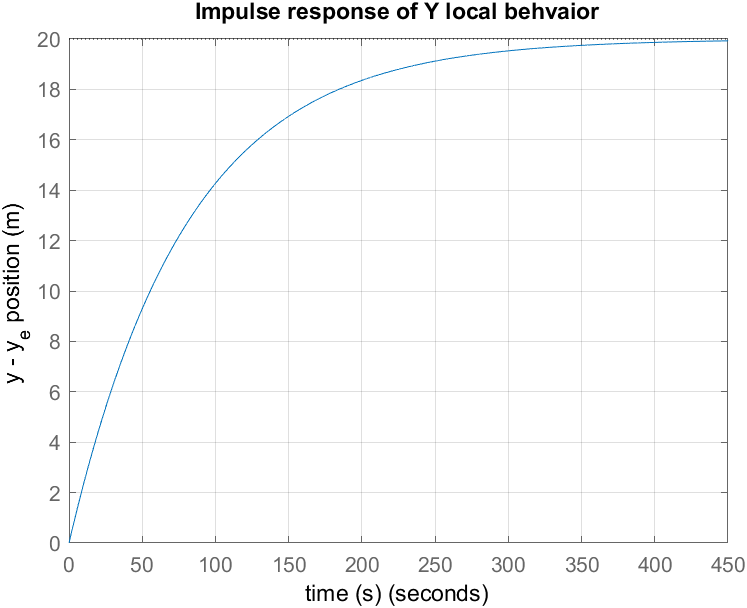
\includegraphics[scale=0.6]{YImpulseRes.png}}
\caption{Impulse Y Position Response}
\label{figure}
\end{figure}

Fig. 9 shows the impulse initially accelerating the aircraft before reaching a steady state position. As previously mentioned, the transfer function predicts an impulse input will behavior like a stable step response. In comparison to the local x response, the local y response is independent of $\theta$ (Equation 22). Therefore, air drag is the only component slowing down the input. \\


\subsubsection{Local Y Step Response} 
\begin{figure}[htbp]
\centerline{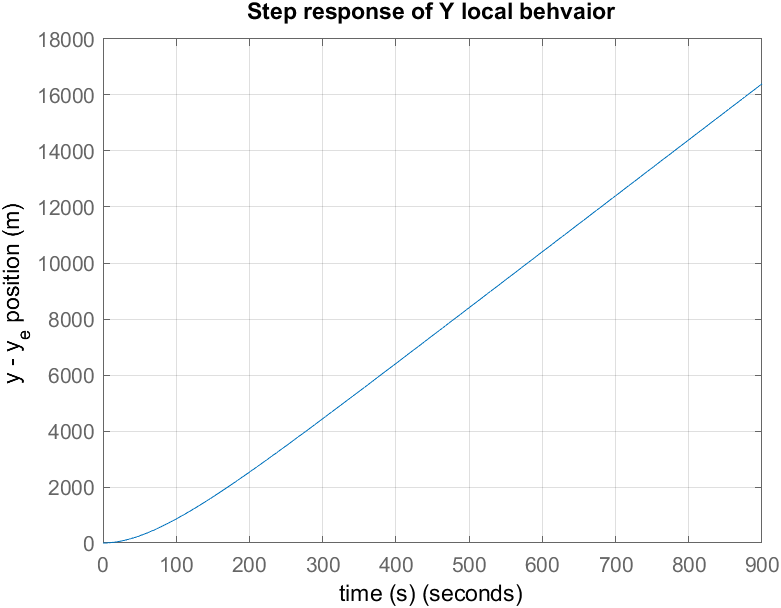
\includegraphics[scale=0.6]{YStepRes.png}}
\caption{Step Y Position Response}
\label{figure}
\end{figure}

In Fig. 10, the local y behavior is linear because the system will reach a constant terminal velocity. Thus, the input is constant and larger than air drag, so this system will tend to positive infinity. As previously mentioned, the local y transfer function shows the step input will behavior like a unstable ramp response. 

\newpage
\subsubsection{Local Y Bode Response} 
\begin{figure}[htbp]
\centerline{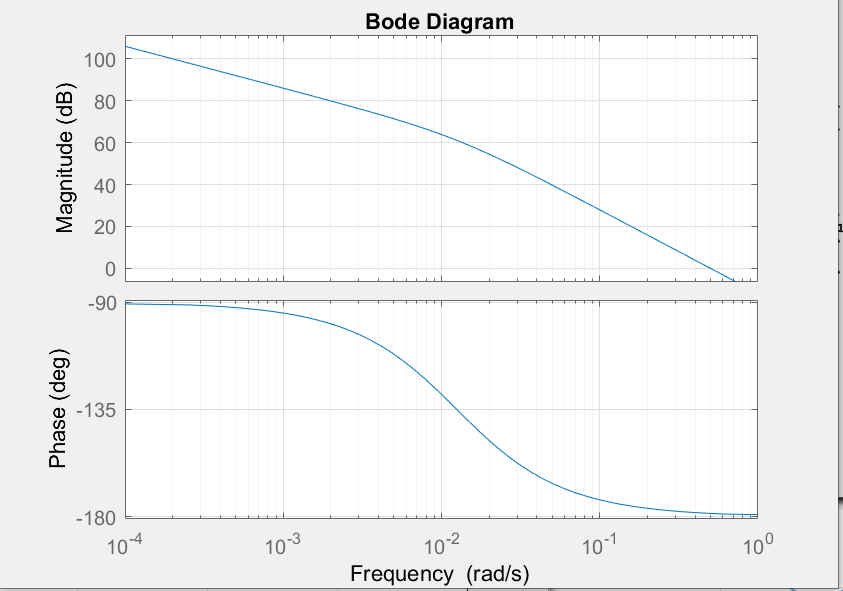
\includegraphics[scale=0.6]{YBode.png}}
\caption{Y Bode Plot}
\label{figure}
\end{figure}

Fig. 11 illustrates the output magnitude at a low frequency is amplified and has a constant slope. At high frequencies, the magnitude slope is constant and steep. The signal will be amplified and then gradually attenuate. The output response is leading the input because the phase plot stays negative. The signal changes from -90$^{\circ}$ phase at low frequencies to a -180$^{\circ}$ phase at high frequencies.

\subsubsection{Local Y High Freq Response} 
\begin{figure}[htbp]
\centering
\centerline{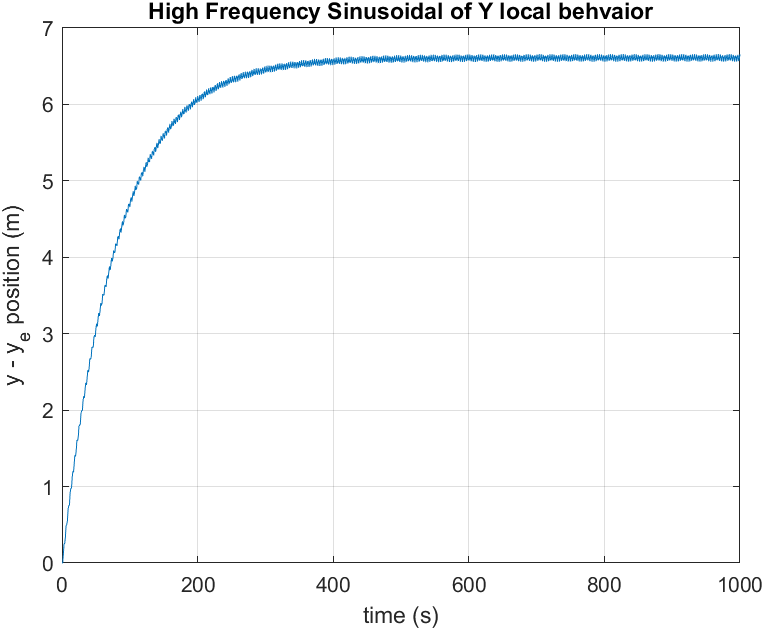
\includegraphics[scale=0.6]{YHighFreqRes.png}}
\caption{High Frequency Sinusoidal Y  Position Responsee}
\label{figure}
\end{figure}

Fig. 12 shows a high frequency response is similar to the impulse response.  
At high frequencies, the local y response will initially be amplified and eventually attenuate around a steady-state value. The system reaches a steady-state value because air drag is slowing down the aircraft. \\

\newpage
\subsubsection{Local Y Low Freq Response} 
\begin{figure}[htbp]
\centerline{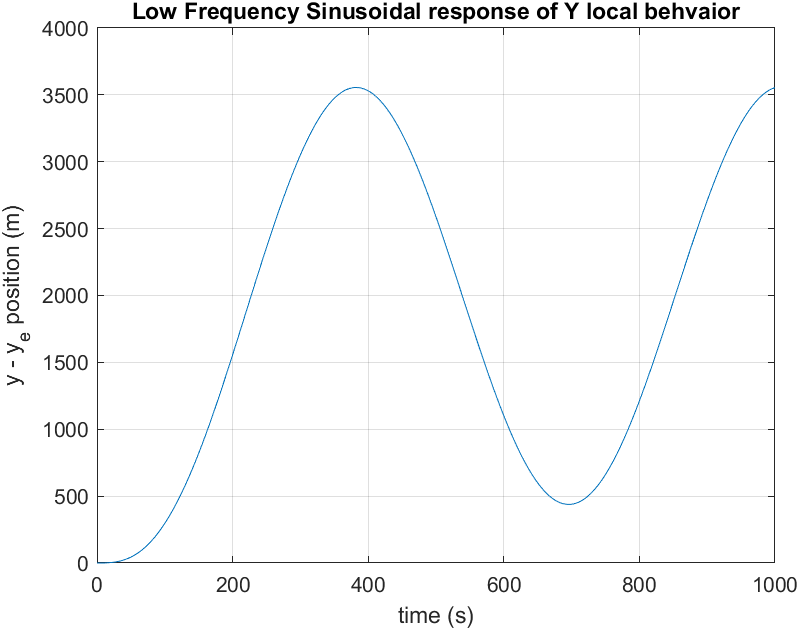
\includegraphics[scale=0.6]{YLowFreqRes.png}}
\caption{Low Frequency Sinusoidal Y Position Response}
\label{figure}
\end{figure}

For low frequencies, the output signal will be amplified and slowly decrease its amplification over time (Fig. 13).  This response converges faster to a steady-state mean than the high frequencies because the Bode Plot slope changes at the simulated frequency. \\


\section{Limitations and Future Improvements}
The limitations of the model are neglecting air torque resistance and reaching beyond the small angle approximation. Note that linearizing the system around its equilibrium points may not capture majority of the nonlinear system dynamics. For future application, a LQR controller can be implemented to control external disturbances and stability. The model can include vertical takeoff and landing maneuvers.

\newpage
\section{Group Contribution Breakdown}
Reese: FBD, Nonlinear and Linear Simulink Models, Block Diagram photos, and interpretation/analysis of the Linear/Nonlinear results to the physical system.\\

Sayed: Nonlinear Simulink model, Linearizing Nonlinear System, Analysis, and Mathematical reviewer.  \\

Tyler: Linearizing Nonlinear System, References, Analysis, MATLAB Simulation, and create Overleaf template with Model equations, Analysis, Simulation, and MATLAB Results. \\

\section{References}
\noindent [1] K. J. Åström, R. M. Murray, \textit{Feedback Systems: An Introduction for Scientists and Engineers.} Princeton University Press, 2008. [Online]. Available: http://www.cds.caltech.edu/$\sim$murray/books/AM08/pdf/fbs-public\_24Jul2020.pdf. 
Accessed: Feb. 10, 2024. \\

\noindent [2] A. D. Lewis and D. R. Tyner, “Geometric Jacobian linearization and LQR theory,” Journal of Geometric Mechanics, vol. 2, no. 4, pp. 397–440, 2010, Accessed on: Feb. 10, 2024. [Online]. Available: https://doi.org/10.3934/jgm.2010.2.397. \\

\noindent [3] K.K. S. Kumar, H. Arya, A. Joshi, "Automatic Control of Harrier Maneuver of an Agile Fixed-Wing UAV," Indian Control Conference (ICC), IEEE, 2019. Accessed on: Feb. 10, 2024. [Online]. Available: https://ieeexplore.ieee.org/document/8715566. \\
\end{document}